\documentclass[10pt]{article}  

%%%%%%%% PREÁMBULO %%%%%%%%%%%%
\title{Reporte de Laboratorio}
\usepackage[spanish]{babel} %Indica que escribiermos en español
\usepackage[utf8]{inputenc} %Indica qué codificación se está usando ISO-8859-1(latin1)  o utf8  
\usepackage{amsmath} % Comandos extras para matemáticas (cajas para ecuaciones,
% etc)
\usepackage{amssymb} % Simbolos matematicos (por lo tanto)
\usepackage{longtable} %agregadom para hacer tablas
\usepackage{xltabular}
\usepackage{graphicx} % Incluir imágenes en LaTeX
\usepackage{color} % Para colorear texto
\usepackage{subfigure} % subfiguras
\usepackage{float} %Podemos usar el especificador [H] en las figuras para que se
% queden donde queramos
\usepackage{capt-of} % Permite usar etiquetas fuera de elementos flotantes
% (etiquetas de figuras)
\usepackage{sidecap} % Para poner el texto de las imágenes al lado
	\sidecaptionvpos{figure}{c} % Para que el texto se alinie al centro vertical
\usepackage{caption} % Para poder quitar numeracion de figuras
\usepackage{commath} % funcionalidades extras para diferenciales, integrales,
% etc (\od, \dif, etc)
\usepackage{cancel} % para cancelar expresiones (\cancelto{0}{x})
 
\usepackage{anysize} 					% Para personalizar el ancho de  los márgenes
\marginsize{2cm}{2cm}{2cm}{2cm} % Izquierda, derecha, arriba, abajo

\usepackage{appendix}
\renewcommand{\appendixname}{Apéndices}
\renewcommand{\appendixtocname}{Apéndices}
\renewcommand{\appendixpagename}{Apéndices} 
% Para que las referencias sean hipervínculos a las figuras o ecuaciones y
% aparezcan en color
\usepackage[colorlinks=true,plainpages=true,citecolor=blue,linkcolor=blue]{hyperref}
%\usepackage{hyperref} 
% Para agregar encabezado y pie de página
\usepackage{fancyhdr} 
\pagestyle{fancy}
\fancyhf{}
\fancyhead[L]{\footnotesize UNI} %encabezado izquierda
\fancyhead[R]{\footnotesize Fac. de Ciencias}   % dereecha
\fancyfoot[R]{\footnotesize Reporte}  % Pie derecha
\fancyfoot[C]{\thepage}  % centro
\fancyfoot[L]{\footnotesize Reporte de conteo y medicion.}  %izquierda
\renewcommand{\footrulewidth}{0.4pt}


\usepackage{listings} % Para usar código fuente
\definecolor{dkgreen}{rgb}{0,0.6,0} % Definimos colores para usar en el código
\definecolor{gray}{rgb}{0.5,0.5,0.5} 
% configuración para el lenguaje que queramos utilizar
\lstset{language=Matlab,
   keywords={break,case,catch,continue,else,elseif,end,for,function,
      global,if,otherwise,persistent,return,switch,try,while},
   basicstyle=\ttfamily,
   keywordstyle=\color{blue},
   commentstyle=\color{red},
   stringstyle=\color{dkgreen},
   numbers=left,
   numberstyle=\tiny\color{gray},
   stepnumber=1,
   numbersep=10pt,
   backgroundcolor=\color{white},
   tabsize=4,
   showspaces=false,
   showstringspaces=false}

\newcommand{\sen}{\operatorname{\sen}}	% Definimos el comando \sen para el seno
%en español

\title{Plantilla para Reportes IMEC-UTB}
% Basada en la plantilla para reportes UPIITA de  Overleaf

%%%%%%%% TERMINA PREÁMBULO %%%%%%%%%%%%

\begin{document}

%%%%%%%%%%%%%%%%%%%%%%%%%%%%%%%%%% PORTADA %%%%%%%%%%%%%%%%%%%%%%%%%%%%%%%%%%%%%%%%%%%%
																					%%%
\begin{center}																		%%%
\newcommand{\HRule}{\rule{\linewidth}{0.5mm}}									%%%\left
 																					%%%
\begin{minipage}{0.48\textwidth} \begin{flushleft}

\includegraphics[scale = 0.9]{Imagenes/UNI_2.png}
\end{flushleft}\end{minipage}
\begin{minipage}{0.48\textwidth} \begin{flushright}

\includegraphics[scale = 0.075]{Imagenes/UNI.png}
\end{flushright}\end{minipage}

													 								%%%
\vspace*{1.0cm}								%%%
																					%%%	
\textsc{\huge Universidad Nacional de Ingieneria }\\[1.5cm]	


\begin{minipage}{0.9\textwidth} 
\begin{center}																					%%%
\textsc{\LARGE Reporte  01 }
\end{center}
\end{minipage}\\[0.5cm]
%%%
    																				%%%
 			\vspace*{1cm}																		%%%
																					%%%
\HRule \\[0.4cm]																	%%%
{ \huge \bfseries Laboratorio de Física I}\\[0.4cm]	%%%
 																					%%%
\HRule \\[1.5cm]																	%%%
 																				%%%
																					%%%
\begin{minipage}{0.46\textwidth}													%%%
\begin{flushleft} \large															%%%

% Aqui a continuación pongan los nombres de los integrantes
\emph{El grupo conformado por:}\\	
Rocca Cruz Axel Benjamin \\
Llactahuaman Quispe Benjamin Israel \\
 Cortez Núñez Christian 


%%%
			%\vspace*{2cm}	
            													%%%
										 						%%%
\end{flushleft}																		%%%
\end{minipage}		
																%%%
\begin{minipage}{0.52\textwidth}		
\vspace{-0.6cm}											%%%
\begin{flushright} \large															%%%
\emph{Profesores:} \\																	%%%
 Tello Gálvez Julio César\\
Brocca Pobes Manuel Enrique%%%
\end{flushright}																	%%%
\end{minipage}	
\vspace*{1cm}
%\begin{flushleft}
 	
%\end{flushleft}
%%%
 		\flushleft{\textbf{\Large Física BFI01}	}\\																		%%%
\vspace{2cm} 																				
\begin{center}	
{\large \today}																	%%%
 			\end{center}												  						
\end{center}							 											
																					
\newpage																		
%%%%%%%%%%%%%%%%%%%% TERMINA PORTADA %%%%%%%%%%%%%%%%%%%%%%%%%%%%%%%%

\tableofcontents 

\newpage

\begin{abstract}
    El desarrollo de este primer laboratorio de física está enfocado al estudio de los distintos procesos de medición y de guiar al estudiante a experimentar la inevitable aparición de errores o incertidumbres en cualquier medición y a aprender a tratar con ellos al momento de operar los resultados.
La metodología de trabajo del laboratorio Nº 01 ha sido dividida en tres partes, siendo estas las siguientes:
\begin{itemize}
    \item Medición y error experimental
    \item Medición y propagación de errores 
    \item Gráfica de los resultados en una medición experimental 
\end{itemize}
 
\end{abstract}

\section{Medición y Error Experimental Con Frijoles}
\subsection{Objetivos}
\begin{itemize}
    \item Determinar la incertidumbre en el siguiente proceso de medición.
    \item Determinar la curva de distribución normal en un proceso de medición, correspondiente al numero de frijoles que caben en vaso seleccionado previamente.
\end{itemize}

\subsection{Fundamento teórico}
\begin{itemize}
    \item \textbf{Medición:} La medición es un proceso básico de la ciencia que se basa en comparar
una unidad de medida seleccionada con el objeto o fenómeno cuya magnitud física se
desea medir, para averiguar cuantas veces la unidad está contenida en esa magnitud.
    \item \textbf{Incertidumbre :} Es el parámetro asociado con el resultado de una medición, que
caracteriza la dispersión de los valores que podrían ser razonablemente atribuidos al
valor a medir. Por ejemplo: Un experimentador que haga la misma medición muchas
veces no obtendrá los mismos resultados tanto por factores externos como (luz, viento,
etc.) como las variaciones en las condiciones de observación del experimentador.
\item \textbf{Ajuste de Curva: } El ajuste de curvas consiste en encontrar una curva que contenga
una serie de puntos y que posiblemente cumpla una serie de restricciones adicionales.
Esta sección es una introducción tanto a la interpolación (cuando se espera un ajuste
exacto a determinadas restricciones) y al ajuste de curvas/análisis de regresión (cuando
se permite una aproximación).
\end{itemize}
\subsection{Materiales y equipos de trabajo}

    \begin{figure}[H]
	\begin{center}
 		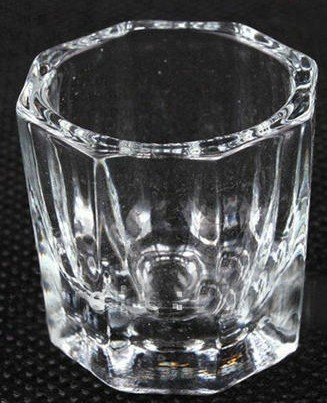
\includegraphics[width = 0.3\textwidth]{Imagenes/vaso.jpg}
 		\captionof{figure}{\label{fig:vaso}vaso pequeño} 
	\end{center} 
    \end{figure}
    \begin{figure}[H]
	\begin{center}
 		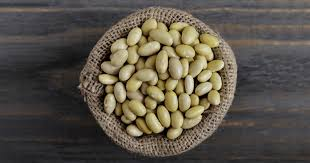
\includegraphics[width = 0.4\textwidth]{Imagenes/frijoles.jpeg}
 		\captionof{figure}{\label{fig:frijoles}frijoles 250gr} 
	\end{center} 
    \end{figure}

\subsection{Resultados y Procedimientos}



\subsubsection{Procedimientos}

\begin{enumerate}
    \item Colocar el vaso sobre una mesa
    \item Vaciar los frejoles en el vaso hasta que se llene. Que no rebase el tope o se aleje mucho de él.
    \item Contar el número de frejoles, devolverlo a la bolsa y sacudirla (Para de evitar sacar los mismos frijoles)
    \item Escribir los resultados en una tabla de (4x100), donde las columnas se encabezan por:
    \begin{itemize}
        \item $K$ : k- esimo conteo 
        \item $N_k$ : el K-esimo conteo de frijoles
        \item $N_k - \overline{mnp}$ :  k-esimo conteo - el promedio 
        \item $(N_k - \overline{mnp})^2$ : k-esimo conteo - el promedio, al cuadrado
    \end{itemize}
    \item Repetir hasta tener 100 repeticiones en total
    \item Determinar la media aritmética $\overline{mnp}$ de los 100 números obtenidos. Esta media aritmética es el número más probable de frijoles que caben en el vaso.

    Sea $N_k$ el número de frijoles obtenidos en la k-ésima operación. La media aritmética de los 100 números obtenidos es:
    \begin{equation*}
        \overline{mnp}=\dfrac{1}{100}\sum_{i=1}^{100} N_k = 144.86
    \end{equation*}
    \item Determine la incertidumbre normal o desviación estándar,$\Delta(\overline{mnp})$ , de la medición anterior.

    La incertidumbre normal o desviación estándar será:
    \begin{equation*}
    \Delta(\overline{n m p})=\sqrt{\frac{1}{100} \sum_{k=1}^{100}\left(N_k-\overline{mnp}\right)^2}=4.622
    \end{equation*}
    \item Grafique tanto la posibilidad $n(r,r+1)$ y $n(r,r+2)$

\end{enumerate}

\newpage
\subsubsection{Resultados} 

\begin{xltabular}{\textwidth}{|c|c|c|c|}
\caption{tabla de resultados de conteo} \label{tab:long} \\

\hline \multicolumn{1}{|c|}{\textbf{K}} & \multicolumn{1}{c|}{\textbf{$N_k$}} & \multicolumn{1}{c|}{\textbf{$N_k - \overline{mnp} $}} & \multicolumn{1}{c|}{\textbf{$(N_k - \overline{mnp})^2$}} \\ \hline 
\endfirsthead

\multicolumn{3}{c}%
{} \\
\hline 
\endhead

\hline \multicolumn{4}{|r|}{{Continued on next page}} \\ \hline
\endfoot

\hline
\endlastfoot

1   & 145 & 0,14  & 0,02  \\
2   & 144 & -0,86 & 0,74  \\
3   & 154 & 9,14  & 83,54 \\
4   & 145 & 0,14  & 0,02  \\
5   & 150 & 5,14  & 26,42 \\
6   & 139 & -5,86 & 34,34 \\
7   & 143 & -1,86 & 3,46  \\
8   & 140 & -4,86 & 23,62 \\
9   & 143 & -1,86 & 3,46  \\
10  & 144 & -0,86 & 0,74  \\
11  & 146 & 1,14  & 1,30  \\
12  & 152 & 7,14  & 50,98 \\
13  & 148 & 3,14  & 9,86  \\
14  & 144 & -0,86 & 0,74  \\
15  & 151 & 6,14  & 37,70 \\
16  & 150 & 5,14  & 26,42 \\
17  & 148 & 3,14  & 9,86  \\
18  & 152 & 7,14  & 50,98 \\
19  & 149 & 4,14  & 17,14 \\
20  & 145 & 0,14  & 0,02  \\
21  & 143 & -1,86 & 3,46  \\
22  & 144 & -0,86 & 0,74  \\
23  & 146 & 1,14  & 1,30  \\
24  & 143 & -1,86 & 3,46  \\
25  & 142 & -2,86 & 8,18  \\
26  & 144 & -0,86 & 0,74  \\
27  & 143 & -1,86 & 3,46  \\
28  & 147 & 2,14  & 4,58  \\
29  & 150 & 5,14  & 26,42 \\
30  & 149 & 4,14  & 17,14 \\
31  & 152 & 7,14  & 50,98 \\
32  & 146 & 1,14  & 1,30  \\
33  & 151 & 6,14  & 37,70 \\
34  & 141 & -3,86 & 14,90 \\
35  & 148 & 3,14  & 9,86  \\
36  & 148 & 3,14  & 9,86  \\
37  & 146 & 1,14  & 1,30  \\
38  & 150 & 5,14  & 26,42 \\
39  & 146 & 1,14  & 1,30  \\
40  & 149 & 4,14  & 17,14 \\
41  & 146 & 1,14  & 1,30  \\
42  & 148 & 3,14  & 9,86  \\
43  & 147 & 2,14  & 4,58  \\
44  & 153 & 8,14  & 66,26 \\
45  & 145 & 0,14  & 0,02  \\
46  & 147 & 2,14  & 4,58  \\
47  & 147 & 2,14  & 4,58  \\
48  & 142 & -2,86 & 8,18  \\
49  & 154 & 9,14  & 83,54 \\
50  & 143 & -1,86 & 3,46  \\
51  & 146 & 1,14  & 1,30  \\
52  & 145 & 0,14  & 0,02  \\
53  & 147 & 2,14  & 4,58  \\
54  & 137 & -7,86 & 61,78 \\
55  & 144 & -0,86 & 0,74  \\
56  & 143 & -1,86 & 3,46  \\
57  & 145 & 0,14  & 0,02  \\
58  & 138 & -6,86 & 47,06 \\
59  & 136 & -8,86 & 78,50 \\
60  & 142 & -2,86 & 8,18  \\
61  & 141 & -3,86 & 14,90 \\
62  & 138 & -6,86 & 47,06 \\
63  & 153 & 8,14  & 66,26 \\
64  & 145 & 0,14  & 0,02  \\
65  & 148 & 3,14  & 9,86  \\
66  & 145 & 0,14  & 0,02  \\
67  & 146 & 1,14  & 1,30  \\
68  & 144 & -0,86 & 0,74  \\
69  & 142 & -2,86 & 8,18  \\
70  & 140 & -4,86 & 23,62 \\
71  & 141 & -3,86 & 14,90 \\
72  & 140 & -4,86 & 23,62 \\
73  & 145 & 0,14  & 0,02  \\
74  & 139 & -5,86 & 34,34 \\
75  & 145 & 0,14  & 0,02  \\
76  & 147 & 2,14  & 4,58  \\
77  & 146 & 1,14  & 1,30  \\
78  & 149 & 4,14  & 17,14 \\
79  & 139 & -5,86 & 34,34 \\
80  & 147 & 2,14  & 4,58  \\
81  & 144 & -0,86 & 0,74  \\
82  & 146 & 1,14  & 1,30  \\
83  & 150 & 5,14  & 26,42 \\
84  & 152 & 7,14  & 50,98 \\
85  & 140 & -4,86 & 23,62 \\
86  & 151 & 6,14  & 37,70 \\
87  & 147 & 2,14  & 4,58  \\
88  & 141 & -3,86 & 14,90 \\
89  & 137 & -7,86 & 61,78 \\
90  & 144 & -0,86 & 0,74  \\
91  & 140 & -4,86 & 23,62 \\
92  & 139 & -5,86 & 34,34 \\
93  & 138 & -6,86 & 47,06 \\
94  & 142 & -2,86 & 8,18  \\
95  & 141 & -3,86 & 14,90 \\
96  & 138 & -6,86 & 47,06 \\
97  & 141 & -3,86 & 14,90 \\
98  & 145 & 0,14  & 0,02  \\
99  & 138 & -6,86 & 47,06 \\
100 & 137 & -7,86 & 61,78 \\
\end{xltabular}

\begin{xltabular}{\textwidth}{|c|c|c|}
    \caption{tabla de posibilidad de $n(r,r+1)$} \label{tab:long} \\

    \hline \multicolumn{1}{|c|}{\textbf{Número de frijoles}} & \multicolumn{1}{c|}{\textbf{$n(r,r+1)$}} & \multicolumn{1}{c|}{\textbf{$\pi(r,r+1)$}}  \\ \hline 
    \endfirsthead

    \multicolumn{3}{c}%
    {} \\
    \hline 
    \endhead

    \hline \multicolumn{3}{|r|}{{Continued on next page}} \\ \hline
    \endfoot

    \hline
    \endlastfoot
    136 & 1  & 0,01 \\ 
    137 & 3  & 0,03 \\ 
    138 & 5  & 0,05 \\ 
    139 & 4  & 0,04 \\ 
    140 & 5  & 0,05 \\ 
    141 & 6  & 0,06 \\ 
    142 & 5  & 0,05 \\ 
    143 & 7  & 0,07 \\ 
    144 & 9  & 0,09 \\ 
    145 & 11 & 0,11 \\ 
    146 & 10 & 0,1  \\ 
    147 & 8  & 0,08 \\ 
    148 & 6  & 0,06 \\ 
    149 & 4  & 0,04 \\ 
    150 & 5  & 0,05 \\ 
    151 & 3  & 0,03 \\ 
    152 & 4  & 0,04 \\ 
    153 & 2  & 0,02 \\ 
    154 & 2  & 0,02 \\ \hline
    \end{xltabular}

    \begin{xltabular}{\textwidth}{|c|c|c|}
    \caption{tabla de posibilidad de $n(r,r+2)$} \label{tab:long} \\

    \hline \multicolumn{1}{|c|}{\textbf{Número de frijoles}} & \multicolumn{1}{c|}{\textbf{$n(r,r+2)$}} & \multicolumn{1}{c|}{\textbf{$\pi(r,r+1)$}}  \\ \hline 
    \endfirsthead

    \multicolumn{3}{c}%
    {} \\
    \hline 
    \endhead

    \hline \multicolumn{3}{|r|}{{Continued on next page}} \\ \hline
    \endfoot

    \hline
    \endlastfoot
    136 - 138 & 4  & 0,04 \\
    138 - 140 & 9  & 0,09 \\
    140 - 142 & 11 & 0,11 \\
    142 - 144 & 12 & 0,12 \\
    144 - 146 & 20 & 0,2  \\
    146 - 148 & 18 & 0,18 \\
    148 - 150 & 10 & 0,1  \\
    150 - 152 & 8  & 0,08 \\
    152 - 154 & 6  & 0,06 \\
    154 - 156 & 2  & 0,02 \hline
\end{xltabular}
\subsection{Preguntas}
\begin{enumerate}
    \item  \textbf{En vez de medir puñados, ¿podría medirse el número de frijoles que caben en
un vaso, en una cuchara, etc.?} 

Sería preferible medir con un vaso ya que el volumen que recogerá se mantendrá relativamente constante. Sobre diferencia entre los puñados se debe a la forma, tamaño y agarre de la mano de cada participante y de su criterio sobre lo que es flojo o apretado. 
    \item. \textbf{Después de realizar los experimentos, ¿qué ventaja le ve a la representación de $\pi [r, r+2)$ frente a la de $\pi [r, r+1)$?}

    A pesar de que esta pierda precisión respecto a [r, r+1), sus resultados mostrados son más consistentes y fáciles de procesar.
    \item  \textbf{¿Qué sucedería si los frijoles fuesen de tamaños apreciablemente diferentes?}
    
    Las mediciones variarían de forma considerable, incluso llegando a resultados drásticamente alejados de la media. 
    \item \textbf{En el ejemplo mostrado se debía contar alrededor de 60 frijoles por puñado. ¿Sería ventajoso colocar solo 100 frijoles en el recipiente, y de esta manera calcular el número de frijoles en un puñado contando los frijoles que quedan en el recipiente?} 
    
    Respecto a la velocidad de medición sería ventajoso realizarlo de esa manera, sin embargo los resultados solo serían confiables respecto a un grupo muy reducido (de 100) en comparación con la muestra original (que sería mucho mayor), debido a que las distintas variaciones dentro de ese grupo podrían ser una representación incorrecta al momento de abarcar una muestra mayo
    \item \textbf{¿Qué sucedería si en el caso anterior colocara solo, digamos 75 frijoles en el
recipiente?} 

    La variación sería incluso menor que en la medición de 100 frijoles, y los casos donde se repitan los mismos grupos de frijoles serían más probables. 
    \item \textbf{La parte de este experimento que exige ¨más paciencia¨ es el proceso de
contar. Para distribuir esta tarea entre tres personas. ¿Cuál de las sugerencias
propondría Ud.? ¿Por qué?} 

    Usar tres recipientes del mismo tamaño y forma, porque ahí el volumen es constante y la muestra recogida a solo se sujeta a las variaciones de tamaño de los frijoles y no del contenedor (la mano)
    \item \textbf{Mencione tres posibles hechos que observarían si en vez de 100 puñados
extrajeran 1000 puñados.} 

\begin{enumerate}
    \item  La variación estándar será diferente y más fiable
    \item La gráfica de frecuencias se aproximaría más a la campana de gauss
    \item Las mediciones podrían verse afectadas por la fatiga de los participantes si se mantiene el método actual de conteo (1 por 1)
\end{enumerate}
    \item \textbf{¿Cuál es el promedio aritmético de las desviaciones $Nk - \overline{mnp}$ ?}

    El promedio es 0, debido a que hay variaciones positivas y negativas respecto al promedio y al sumarlas todas se anulan mutuamente.
    \item \textbf{¿Cuál cree Ud. es la razón para haber definido $\Delta \overline{mnp}$ en vez de tomar
simplemente el promedio de las desviaciones?}

    La razón fue justamente evitar la anulación del resultado al convertir los valores negativos a positivos y obtener un resultado pertinente.
    \item \textbf{Después de realizar el experimento coja Ud. un puñado de frijoles. ¿Qué puede
Ud. afirmar sobre el número de frijoles contenido en tal puño (antes de contar)?} 

    Se puede afirmar que la cantidad a ser contada será cercana al promedio obtenido
    \item \textbf{Mencione Ud. alguna ventaja o desventaja de emplear pallares en vez de
frijoles en el presente experimento.}

    Como ventaja sería más rápido el conteo, sin embargo por su mayor tamaño y forma irregular respecto a los frejoles crearía mayores espacios de vacío que afectarían a la medición
\end{enumerate}

\cite{IEEEreferencias:Ref2}

\newpage

\section{Propagaci\'on del Error Experimental}

\subsection{Objetivo}
Determinar el error y su propagación por medio de experimentos, al usar distintos instrumentos de medición.

\subsection{Fundamento te\'orico}
\begin{itemize}
    \item \textbf{Medir}: Una medición es comparar la cantidad desconocida que queremos determinar y una cantidad conocida de la misma magnitud, que elegimos como unidad. Al resultado de medir se le denomina medida.
    \item \textbf{Instrumentos de medición}: Es un instrumento que se usa para medir una cantidad física. Los instrumentos de medición se caracterizan por su precisión, exactitud, resolución, apreciación, sensibilidad.
    \item \textbf{Error}: El error de medición es la diferencia que hay entre el valor medido y el valor real. Este puede deberse a diversas causas, entre ellas están los factores ambientales, desgaste o fallo en el diseño del instrumento.
    \item \textbf{Propagación de error}: Es el efecto de variables de incertidumbre en la incertidumbre de una función matemática basada en ellos. Cuando las variables son los valores de mediciones experimentales tienen incertidumbre debido a la medición de limitaciones (por ejemplo, instrumento de precisión), que se propagan a la combinación de variables en la función.
\end{itemize}

\subsection{Materiales}

\begin{figure}[H]
	\begin{center}
 		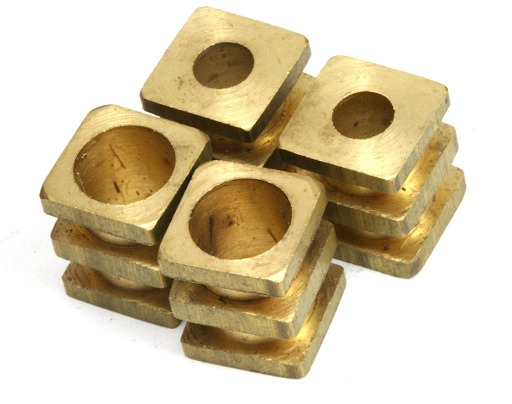
\includegraphics[width = 0.3\textwidth]{Imagenes/para.jpg}
 		\captionof{figure}{\label{fig:paralepipedo de metal}paralepipedo de metal} 
	\end{center} 
\end{figure}

\begin{figure}[H]
	\begin{center}
 		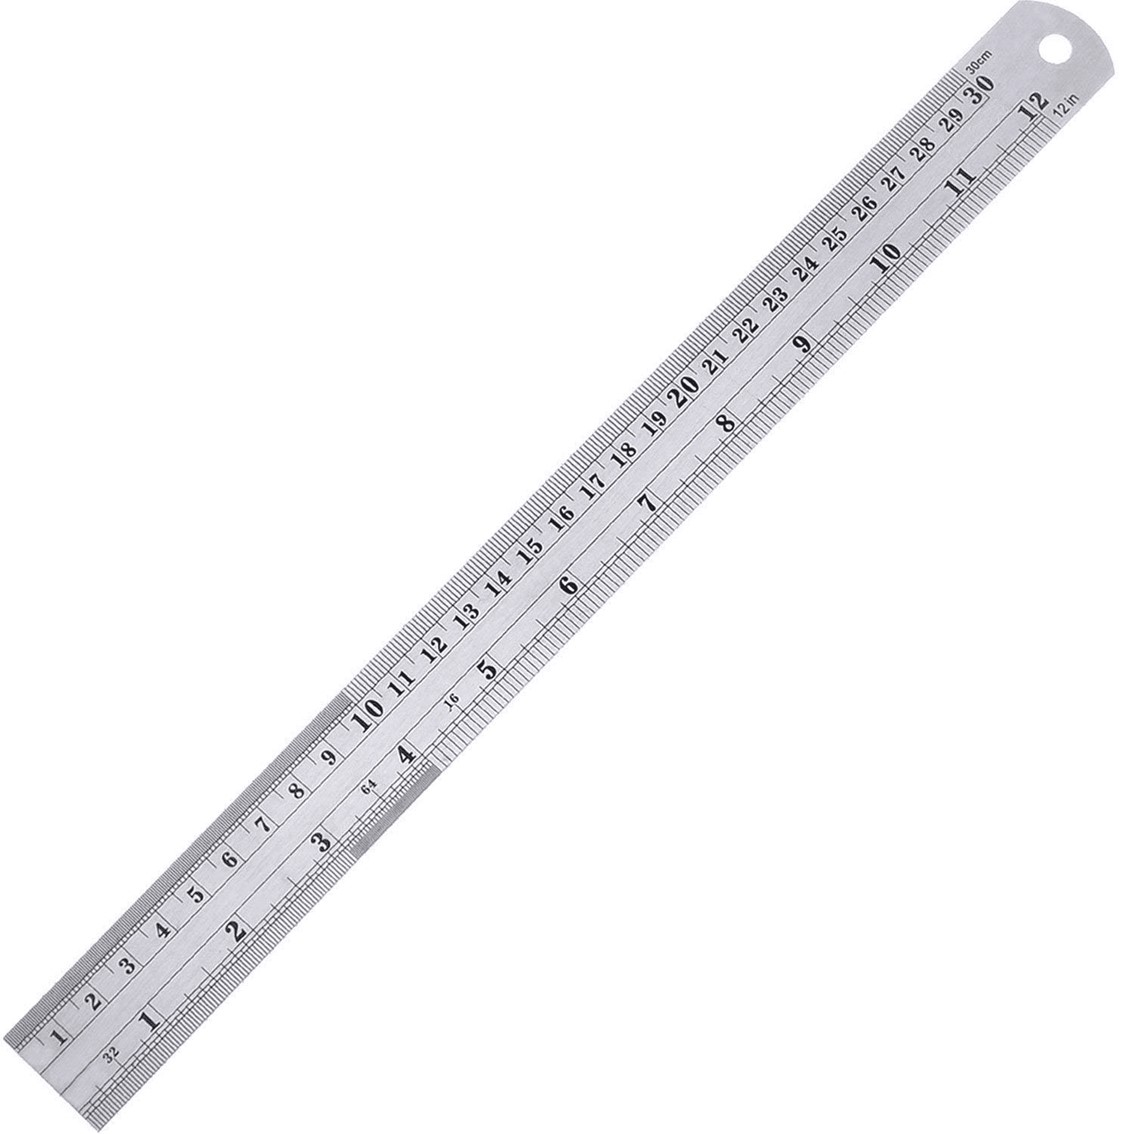
\includegraphics[width = 0.3\textwidth]{Imagenes/regla.jpg}
 		\captionof{figure}{\label{fig:Regla}Regla} 
	\end{center} 
\end{figure}

\begin{figure}[H]
	\begin{center}
 		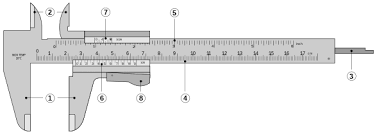
\includegraphics[width = 0.5\textwidth]{Imagenes/vernier.png}
 		\captionof{figure}{\label{fig:pie de rayo  o vernier}pie de rayo  o vernier} 
	\end{center} 
\end{figure}

\subsection{Procedimientos}
\begin{itemize}
    \item Diferenciar entre objeto a medir e instrumentos para medir
    \item Medir las dimensiones del objeto con la regla graduada en milímetros y anotarlas junto al error correspondiente del instrumento.
    \item Medir las dimensiones del objeto con el vernier y anotarlas junto al error correspondiente del instrumento.
    \item Hacer un cuadro que indique las dimensiones, el área y volumen del paralelepípedo medido con la regla y medido con el vernier, indicar sus medidas con su error correspondiente.
    \item suponga que coloca 100 paralepipedo, apoyando uno sobre otro, formando un gran paralepípedo, denotado asi, $A_{100} V_{100}$
\end{itemize}

\subsection{Resultados obtenidos}

\begin{table}[H]
\begin{tabular}{lll}
\cline{1-2}
\multicolumn{1}{|l|}{Incertidumbre de la regla milimetrada:} & \multicolumn{1}{l|}{0,03 cm} &  \\ \cline{1-2}
\multicolumn{1}{|l|}{Incertidumbre del pie de rey:}          & \multicolumn{1}{l|}{0,003}   &  \\ \cline{1-2}
                                                             &                              & 
\end{tabular}
\end{table}



\begin{xltabular}{\textwidth}{|c|c|c|}
    \caption{Medidas con su inceridumbre} \label{tab:long} \\

    \hline \multicolumn{1}{|c|}{} & \multicolumn{1}{c|}{\textbf{Medida de la regla milimetrada}} & \multicolumn{1}{c|}{\textbf{Medida delpie de rey}}  \\ \hline 
    \endfirsthead

    \multicolumn{3}{c}%
    {} \\
    \hline 
    \endhead

    \hline \multicolumn{3}{|r|}{{Continued on next page}} \\ \hline
    \endfoot

    \hline
    \endlastfoot
    Largo (a) & $(3,20 \pm 0,03) cm$                                        & $(3,200 \pm 0,003)cm$                            \\
    Ancho (b) & $(3,19 \pm 0,03)cm$                                        & $(3,195 \pm 0,003)cm$                            \\
    Alto  (h) & $(1,25 \pm 0,03)   cm$                                     & $(1,261 \pm 0,003)cm$                         \\
    Area    (A)      & $(28,90 \pm 0,73)cm^2 $                             & $(29,010 \pm 0,073 )cm^2    $                      \\
    Volumen   (V)       & $(12,76 \pm 0,54)cm^3 $                                 & $(12,892 \pm 0,055)cm^3  $                         \\
    $a_{100}$       & $3,20 \pm 0,03$                                        & $3,200 \pm 0,003               $             \\
    $b_{100}$       & $3,19 \pm 0,03$                                        & $3,195 \pm 0,003          $                  \\
    $h_{100}$       & $125 \pm 3$                                            & $126,1 \pm 0,3 $                             \\
    $A_{100}$       & $1617,92 \pm 53,72$                                    & $1633,267 \pm 4.632 $                        \\
    $V_{100}$       & $1276 \pm 54$                                          & $1289,2 \pm 5,5$            
\end{xltabular}


\begin{itemize}
    \item Cálculo del área total (con la regla)
        \begin{equation*}
            A =2(h)(a+b) + 2(ab)
        \end{equation*}


    \item Cálculo del volumen (con la regla)
        \begin{equation*}
            V = (a)(b)(h) 
        \end{equation*}
        \begin{equation*}
            V=(1,25 \pm 0,03)(3,20 \pm 0,03)(3,19 \pm 0,03)
        = 12,76 \pm 0,54 cm^3
        \end{equation*}


    \item Cálculo de área total (con el pie de rey)
\begin{equation*}
    A=2(h)(a+b) + 2(a)(b) 
\end{equation*}
\begin{equation*}
    A=2(1,261 \pm 0,003)( (3,200 \pm 0,003) + (3,195 \pm 0,003) ) + 2(3,200 \pm 0,003)(3,195 \pm 0,003)
= 29,010 \pm 0,073 cm2
\end{equation*}

    \item Cálculo del volumen (con el pie de rey)
\begin{equation*}
    V=(a)(b)(h)
\end{equation*}
\begin{equation*}
    V=(3,200 \pm 0,003)(3,195 \pm 0,003)(1,261 \pm 0,003)
= 12,892 \pm 0.055 cm3
\end{equation*}

    \item Cálculo de área total de una torre de 100 piezas apiladas 
        \begin{itemize}
            \item Cálculo con regla
    \begin{equation*}
            A_{100}=2(h100)(a+b) + 2(ab)
    \end{equation*}
    \begin{equation*}
        A_{100}=2(125 \pm 3)( (3,20 \pm 0,03) + (3,19 \pm 0,03) ) +2 ( (3,20 \pm 0,03)  (3,19 \pm 0,03) )
        = 1617,92 \pm 53,72 cm2
    \end{equation*}

    \item Cálculo con pie de rey
        \begin{equation*}
            A_{100}=2(h100)(a+b) + 2(ab)
        \end{equation*} 
        \begin{equation*}
            A_{100}=2(126,1 \pm 0,3)( (3,200 \pm 0,003) + (3,195 \pm 0,003) ) + 2(3,200 \pm 0,003)(3,195 \pm 0,003)
        = 1633,267 \pm 4.632 cm2
        \end{equation*}
        \end{itemize}

\end{itemize}

\subsection{Cuestionario}
\begin{enumerate}
    \item \textbf{¿ Las dimensiones de un paralelepípedo se pueden determinar con una sola medición? Si no, ¿ Cuál es el procedimiento más apropiado?}
    
Enfocándonos en la precisión, no sería recomendable realizar una única medición que determine el tamaño de cada lado del paralelepípedo, sino realizar varias mediciones para minimizar el error.
    \item \textbf{¿Qué es más conveniente para calcular el volumen del paralelepípedo: una regla en milímetros o un pie de rey?}

    
Lo más conveniente es el pie de rey debido a su mayor precisión en la medición, en la graduación y la forma de medir, de modo que al calcular el volumen la incertidumbre es mucho menor que con una regla.

\end{enumerate}

\newpage

\section{Medición y error experimental}

\subsection{Objetivos}
\begin{itemize}
	\item Determinar las condiciones para que un péndulo simple tenga su período independiente de su amplitud angular.
	\item Determinar la relación entre el período y la longitud l del péndulo.
	\item Construir funciones polinómicas que representen a dicha función.
\end{itemize}
\subsection{Fundamento Teórico}
\begin{itemize}
	\item \textbf{Período (T):}

	      El período mide el tiempo que se tarde en dar una vuelta completa y se mide en segundos.
	      La unidad del periodo en el S.I. es el segundo(s).
	\item \textbf{Frecuencia (f) :}

	      La frecuencia mide la cantidad de vueltas que se dan en un período de tiempo. La unidad de
	      la frecuencia en el S.I. es el Hertz($s^-1$).
	      \begin{equation*}
		      f=\dfrac{N^{\circ} \text { ciclos }}{t}=\dfrac{1}{T}
	      \end{equation*}
	\item \textbf{Frecuencia angular($w$):}
	      Se refiere a la frecuencia del movimiento circular expresada en proporción del cambio de
	      ángulo, y se define como veces la frecuencia. Se expresa en radianes/Segundo, y formalmente,
	      se define con la letra omega minúscula($w$) a través de la fórmula:
	      \begin{equation*}
		      w=2\pi f=\dfrac{2\pi}T
	      \end{equation*}
	\item \textbf{Osilaciones :}
	      Se dice que es una variación, perturbación o fluctuación en el tiempo de un medio o sistema. Si
	      el fenómeno se repite, se habla de oscilación periódica.
	      Una oscilación, en física, química e ingeniería es el movimiento repetido de un lado a otro en
	      torno a una posición central, o posición de equilibrio. El recorrido que consiste en ir desde una
	      posición extrema a la otra y volver a la primera, pasando dos veces por la posición central, se
	      denomina ciclo. El número de ciclos por segundo, Hertz (Hz), se conoce como frecuencia de la
	      oscilación empleada en el movimiento armónico simple.
	\item \textbf{Movimiento Armónico Simple:}
	      Hay muchas situaciones en física en las cuales la fuerza que siente una partícula en cierto
	      sistema es proporcional a un desplazamiento respecto cierto punto “de equilibrio”. Es decir,
	      existen sistemas para los cuales es válida la ley de Hooke.
	      \begin{equation*}
		      F = -kx
	      \end{equation*}
	\item \textbf{Péndulo:}
	      Existen muy variados tipos de péndulos que, atendiendo a su configuración y usos,
	      reciben los nombres apropiados: péndulo simple, péndulo compuesto, péndulo cicloidal,
	      doble péndulo, péndulo de Foucault, péndulo de Newton, péndulo balístico, péndulo de
	      torsión, péndulo esférico, etcétera.
	\item \textbf{Péndulo Simple}
	      El péndulo simple es un sistema mecánico que se mueve en un movimiento oscilatorio.
	      Un péndulo simple se compone de una masa puntual m suspendida por una cuerda
	      ligera supuestamente inextensible de longitud l, donde el extremo superior de la cuerda
	      está fijo
\end{itemize}
\subsection{Materiales y  equipos de trabajo}
\begin{figure}[H]
	\begin{center}
		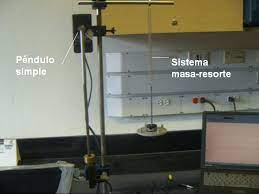
\includegraphics[width = 0.5\textwidth]{Imagenes/pen.jpg}
		\captionof{figure}{pendulo simple}
	\end{center}
\end{figure}

\begin{figure}[H]
	\begin{center}
		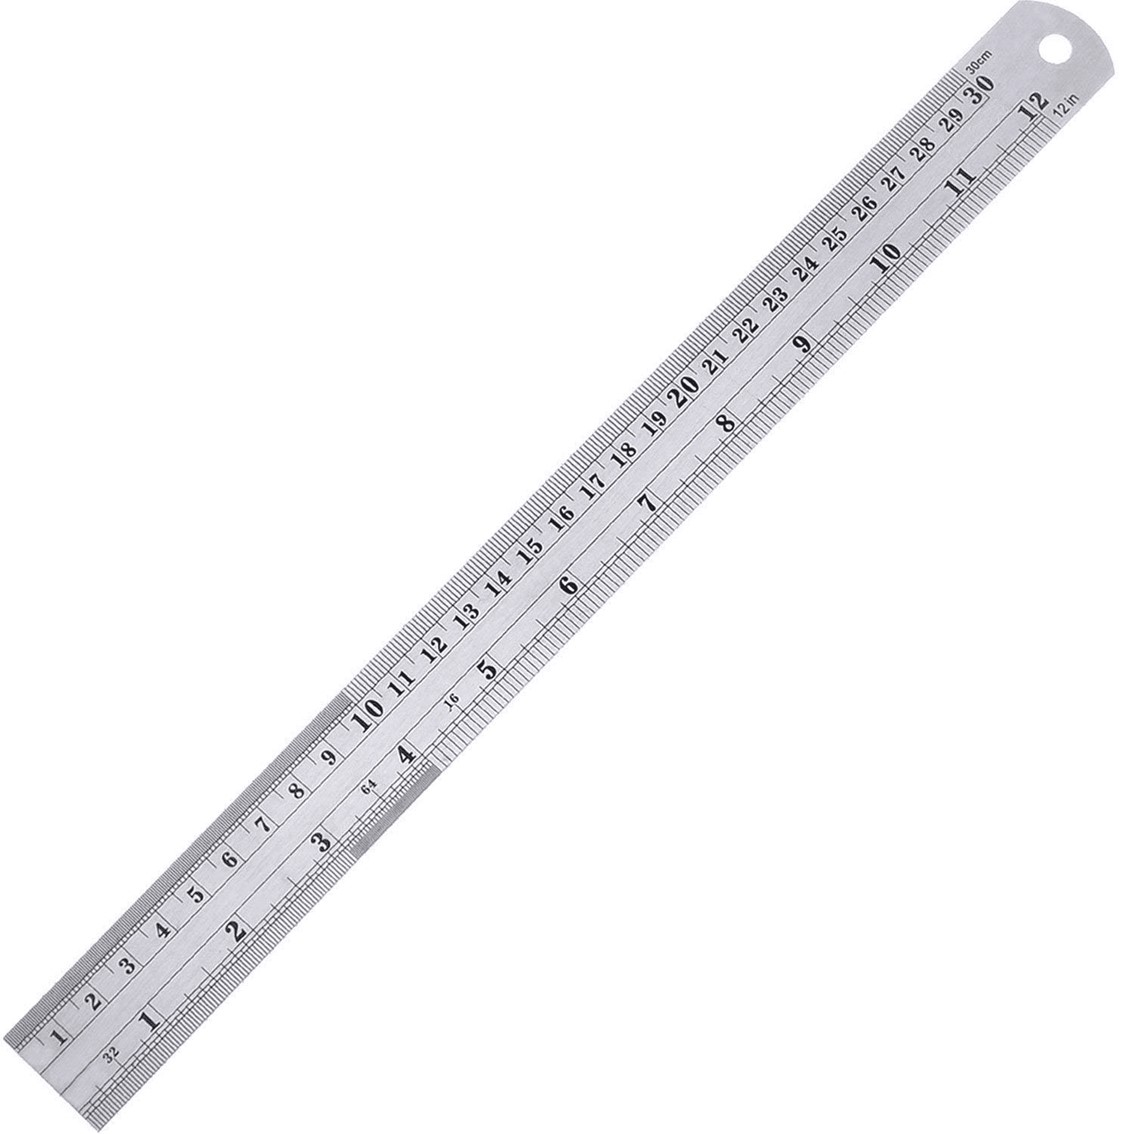
\includegraphics[width = 0.5\textwidth]{Imagenes/regla.jpg}
		\captionof{figure}{una regla}
	\end{center}
\end{figure}

\begin{figure}[H]
	\begin{center}
		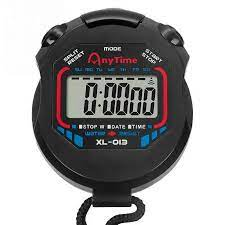
\includegraphics[width = 0.4\textwidth]{Imagenes/crono.jpg}
		\captionof{figure}{un cronometro}
	\end{center}
\end{figure}

\subsection{Procedimientos}
\begin{enumerate}
	\item  Tome la pieza metálica y con la regla, mida tres veces y en lugares diferentes, el largo, el ancho, el alto, el diámetro mayor y el diámetro menor de los agujeros de la pieza.
	\item Tome la pieza metálica y con el pie de rey, mida tres veces y en lugares diferentes, el largo, el ancho, el alto, el diámetro mayor, el diámetro menor, la altura mayor del agujero y la altura menor del agujero.
	\item Determine la incertidumbre de la regla y del pie de rey.
	\item Con las mediciones realizadas y sus incertidumbres, calcule el  área lateral (es decir la suma de las áreas de las caras donde no está el agujero) de la pieza con su incertidumbre respectiva.

\end{enumerate}
\subsection{Resultados Obtenidos}


\begin{xltabular}{\textwidth}{|c|c|}
	\caption{Tabla de Incertidumbre humana} \\

	\hline \multicolumn{1}{|c|}{\textbf{Activación del cronómetro}} & \multicolumn{1}{c|}{\textbf{Tiempo}}  \\ \hline
	\endfirsthead

	\multicolumn{2}{c}%
	{} \\
	\hline
	\endhead

	\hline \multicolumn{2}{|r|}{{Continued on next page}} \\ \hline
	\endfoot

	\hline
	\endlastfoot
	1                         & 0,23                         \\
	2                         & 0,2                          \\
	3                         & 0,18                        \\
	4                         & 0,21                         \\
	5                         & 0,18                         \\
	6                         & 0,15                         \\ \hline
	Promedio (incertidumbre)  & 0,19
\end{xltabular}



\begin{xltabular}{\textwidth}{|c|c|c|c|c|c|c|c|}
	\caption{Tabla de resultados de medición del Periodo} \\

	\hline \multicolumn{1}{|c|}{K} & \multicolumn{1}{c|}{\textbf{L(cm)}} & \multicolumn{1}{c|}{\textbf{$T_1$}} & \multicolumn{1}{c|}{\textbf{$T_2$}} & \multicolumn{1}{c|}{\textbf{$T_3$}} & \multicolumn{1}{c|}{\textbf{$T_4$}} & \multicolumn{1}{c|}{\textbf{$T_k$}} & \multicolumn{1}{c|}{\textbf{($T_k)^2$}}  \\ \hline
	\endfirsthead

	\multicolumn{8}{c}%
	{} \\
	\hline
	\endhead

	\hline \multicolumn{8}{|r|}{{Continued on next page}} \\ \hline
	\endfoot

	\hline
	\endlastfoot
	1          & 20     & 0,961   & 0,964  & 0,949  & 0,95   & 0,956  & 0,914 \\
	2          & 30     & 1,233   & 1,234  & 1,236  & 1,222  & 1,231  & 1,515 \\
	3          & 40     & 1,343   & 1,345  & 1,347  & 1,34   & 1,34   & 1,796 \\
	4          & 50     & 1,472   & 1,475  & 1,486  & 1,49   & 1,48   & 2,190 \\
	5          & 60     & 1,598   & 1,595  & 1,601  & 1,594  & 1,59   & 2,528 \\
	6          & 70     & 1,716   & 1,725  & 1,721  & 1,724  & 1,72   & 2,958 \\
	7          & 80     & 1,847   & 1,84   & 1,834  & 1,838  & 1,83   & 3,349 \\
	8          & 90     & 1,947   & 1,934  & 1,93   & 1,932  & 1,94   & 3,764 \\
	9          & 100    & 2,042   & 2,037  & 2,031  & 2,031  & 2,04   & 4,162
\end{xltabular}


\textbf{Representación polinómica de los resultados Método:} Ajuste lineal por mínimos cuadrados




\begin{enumerate}
	\item Preparación de los valores implicados en la operación







	      \begin{xltabular}{\textwidth}{|c|c|c|c|c|c|c|c|}
		      \caption{Tabla de resultados de medición del Periodo} \\

		      \hline \multicolumn{1}{|c|}{} & \multicolumn{1}{c|}{\textbf{x}} & \multicolumn{1}{c|}{\textbf{y}} & \multicolumn{1}{c|}{\textbf{$xy$}} & \multicolumn{1}{c|}{\textbf{$x^2$}} & \multicolumn{1}{c|}{\textbf{$y^2$}}   \\ \hline
		      \endfirsthead

		      \multicolumn{6}{c}%
		      {} \\
		      \hline
		      \endhead

		      \hline \multicolumn{6}{|r|}{{Continued on next page}} \\ \hline
		      \endfoot

		      \hline
		      \endlastfoot
		      & 20  & 0,914  & 18,28   & 400,000   & 0,835  \\
		      & 30  & 1,515  & 45,45   & 900,000   & 2,295  \\
		      & 40  & 1,796  & 71,84   & 1600,000  & 3,226  \\
		      & 50  & 2,190  & 109,5   & 2500,000  & 4,796  \\
		      & 60  & 2,528  & 151,68  & 3600,000  & 6,391  \\
		      & 70  & 2,958  & 207,06  & 4900,000  & 8,750  \\
		      & 80  & 3,349  & 267,92  & 6400,000  & 11,216 \\
		      & 90  & 3,764  & 338,76  & 8100,000  & 14,168 \\
		      & 100 & 4,162  & 416,2   & 10000,000 & 17,322 \\ \hline
		      Sumatorias         & 540 & 23,176 & 1626,69 & 38400,000 & 68,999 \\  \hline
		      Media              & 60  & 2,575 & & &
	      \end{xltabular}

	\item Operciones

	      \begin{equation*}
		      m=\dfrac{n\left(\sum x y\right)-\left(\sum x\right)\left(\sum y\right)}{n\left(\sum x^2\right)-\left(\sum x\right)^2}=0,0394
	      \end{equation*}
	      \begin{equation*}
		      b=\bar{y}-m \bar{x}=0,2138
	      \end{equation*}
	      \begin{equation*}
		      r=\dfrac{n\left(\sum x y\right)-\left(\sum x\right)(\Sigma y)}{\sqrt{\left[n\left[\sum x^2\right)-\left(\sum x\right)^2\right]\left[n\left(\Sigma y^2\right)-(\Sigma y)^2\right]}}=0,9987
	      \end{equation*}
	      \begin{equation*}
		      r^2=(\dfrac{n\left(\sum x y\right)-\left(\sum x\right)(\Sigma y)}{\sqrt{\left[n\left[\sum x^2\right)-\left(\sum x\right)^2\right]\left[n\left(\Sigma y^2\right)-(\Sigma y)^2\right]}})^2=0,9973
	      \end{equation*}

	      \textbf{Entonces la Ecuación de la recta hallada es : $y = 0,03935x + 0,21381$}
	\item De la ecuacion se obtiene y superponiendo las mediciones reales

	      \begin{figure}[H]
		      \begin{center}
			      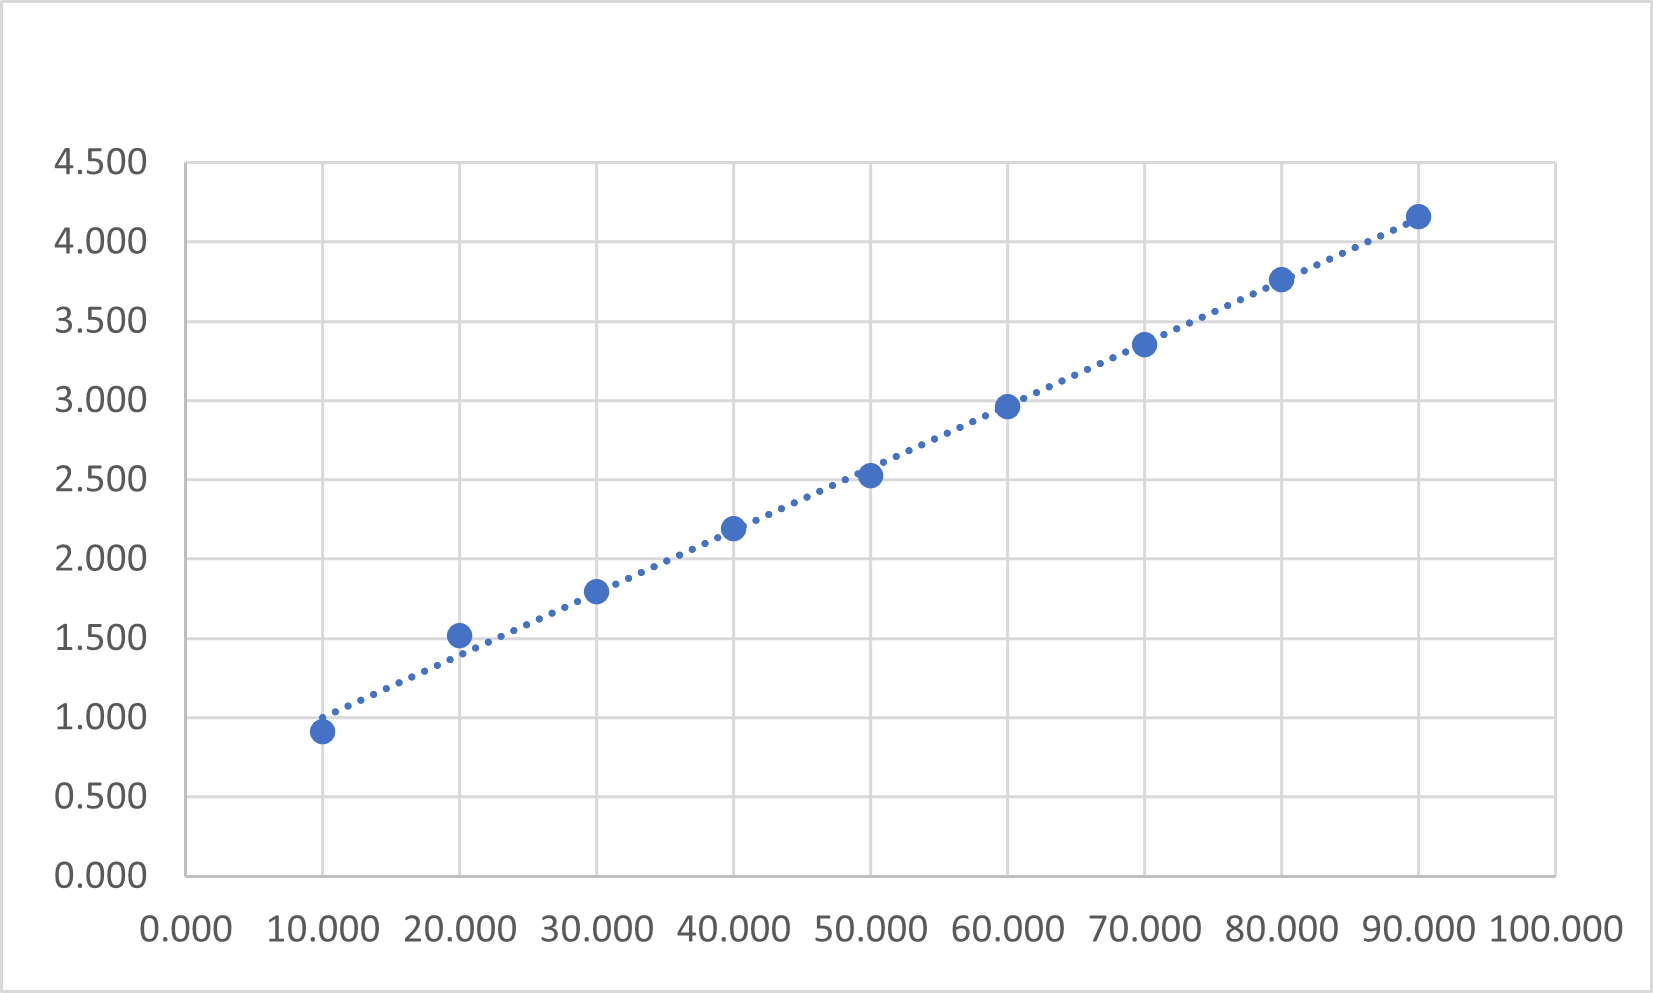
\includegraphics[width = 0.6\textwidth]{Imagenes/Imagen3.png}
			      \captionof{figure}{ del periodo al cuadrado en funcion de la longitud}
		      \end{center}
	      \end{figure}
\end{enumerate}

\subsection{Cuestionario}
\begin{enumerate}
	\item \textbf{Anteriormente se le ha pedido que para medir el periodo suelte la masa del péndulo. ¿Qué sucede si en vez de ello lanza la masa?}

	      Si se lanza la masa, se tendría una aceleración inicial que alteraría considerablemente el periodo de oscilación a medir.
	\item \textbf{¿Depende el per\'iodo del tamaño que tenga la masa? Explique.}


	      Una masa de mayor tamaño no representaría un cambio apreciable a la medición del periodo a pesar de la resistencia del aire, siendo esta mínima. Incluso si se desprecia la resistencia del aire, el periodo sería totalmente independiente del objeto.
	\item \textbf{Para determinar el periodo (duración de una oscilacion completa), se ha pedido medir la duración de 10 oscilaciones y de allí determinar la duración de una oscilación. ¿Por qué no es conveniente medir la duración de una sola oscilación? ¿Qué sucedería si midiera el tiempo necesario para 50 oscilaciones?}
	      \begin{itemize}
		      \item Primero, no es conveniente medir una única oscilación debido al error humano por el tiempo de reacción, mientras que con 10 oscilaciones es posible predecir el fin de una oscilación y así minimizar el error.
		      \item Segundo, podría haber más exactitud en la medición pero es más probable que no llegue a las 50 oscilaciones debido a la resistencia del aire y a eso se podría añadir la fatiga humana de medir 50 oscilaciones por repetición.
	      \end{itemize}

	\item \textbf{¿Cuantas oscilaciones cree que daria el péndulo de longitud 100 cm antes de detenerse?}
	      Aproximadamente unas 40 oscilaciones antes de detenerse
	\item \textbf{Observe que al soltar el p\'endulo es muy dif\'icil evitar que la masa “rote” ¿Modifica tal rotaci\'on el valor del periodo?}
	      Va a modificar el valor del periodo medido porque añade momentum extra, sin embargo esa variación sería despreciable.

\end{enumerate}
\subsection{observaciones}
\begin{enumerate}
	\item Con respecto a la medición de la pieza metálica debemos tomar en cuenta no solo la incertidumbre y el error humano, sino también la forma y disposición de la mesa donde se realiza la medición. por ejemplo sus imperfecciones, como muescas, rayones y deformaciones que pueden afectar los resultados.
	\item La medición de la longitud de la cuerda del péndulo se ve afectada en cierta medida por la elasticidad del material, no solo por la incertidumbre en los instrumentos y el error humano
	\item Las diferentes formas en que se realiza el nudo afectan también a la longitud final del péndulo, ya sea por el ángulo en que se realice o que tan ajustado sea el nudo
	\item la propia masa usada también puede contribuir a la imprecisión debido a que no es una pieza sólida, sino más bien dos piezas unidas que pueden tener algo de movimiento respecto una a la otra (sin embargo es despreciable)
	\item debido a factores como externos como la poca familiaridad con el laboratorio, la programación de un evento que mantenía cierta presión en el horario (la fumigación del laboratorio) e incomodidad general por las alta temperatura, podría verse afectada de forma negativa la capacidad de los participantes para tomar las medidas de forma precisa y consistente.
	\item Los movimientos de los participantes pueden afectar al movimiento del péndulo y a la precisión de las mediciones de la pieza metálica

\end{enumerate}
\subsection{Conclusiones}
\begin{itemize}
	\item Aprender a realizar mediciones de forma precisa y tomando en cuenta tanto la incertidumbre como el error humano es muy importante para estudios científicos debido a que es la base de cualquier experimento.
	\item La manipulación de los instrumentos de medición debe realizarse con cuidado para evitar daños y deformaciones que puedan alterar las mediciones a futuro. Incluso, aunque estas variaciones sean mínimas, al momento de operar resultará en errores más grandes.
	\item La comunicación es sumamente importante al momento de coordinar quienes realizan la experimentación y quienes registrarán los resultados, y cuales son los parámetros base de la experiencia.
	\item Antes de la realización del experimento es necesario revisar los materiales a usar y las distintas situaciones y variaciones que estos puedan experimentar. Casos como el uso de una cuerda muy elástica, una mesa irregular, o instrumentos dañados deben evitarse para maximizar la precisión de los resultados.
	\item Es importante seguir las indicaciones que se dan en el laboratorio y tener la guía a mano a fin de evitar retrasos y confusiones que puedan afectar a los resultados obtenidos del experimento o alargar su duración innecesariamente.

\end{itemize}


\section{Bibliografía}
\begin{itemize}
    \item  Serway. F\'isica. Editorial McGraw-Hill (1992).\\
    \item Tipler. Física. Editorial Revert\'e (1994). \\
    \item Taylor, J.R. (2014) Introducci\'on al Análisis de errores - reverte, Taylor 2 Muestra.pdf. Disponible en: https://www.reverte.com/media/reverte/files/book-attachment-3746.pdf (Accessed: April 14, 2023).

\end{itemize}
\end{document}